\chapter{Implementation}

The application is developed in C$++$ using Microsoft's Visual Studio IDE and can run on computers with a Windows operating system. On an implementation level, platform-specific features are used for saving and loading data files and running the GUI. The implementation consist of three big parts: graphical user interface, back-end software and gesture recognition.\\


\section{Graphical user interface}



In this chapter the implementation of the UI is discussed. First the used technologies are given, then the class diagram is discussed per class and last the general flow of the program is described.\\

{\large COMMENT: zou ik deze dislaimer houden? , de UML moet echt veel groter} \\

WPF is used to easily create buttons and input fields to use as a developer's UI seen on the right side of figure \ref{real implementation}. The interface for the actual users is created in the D2Direct. Because this part of the program was used to experiment with different types of feedback and UI elements it had to be made easily adaptable, for this reason it uses structures that are commonly seen as bad practice like global instances of classes and loosely defined class roles.  

\begin{figure}[H]
	\begin{center}
		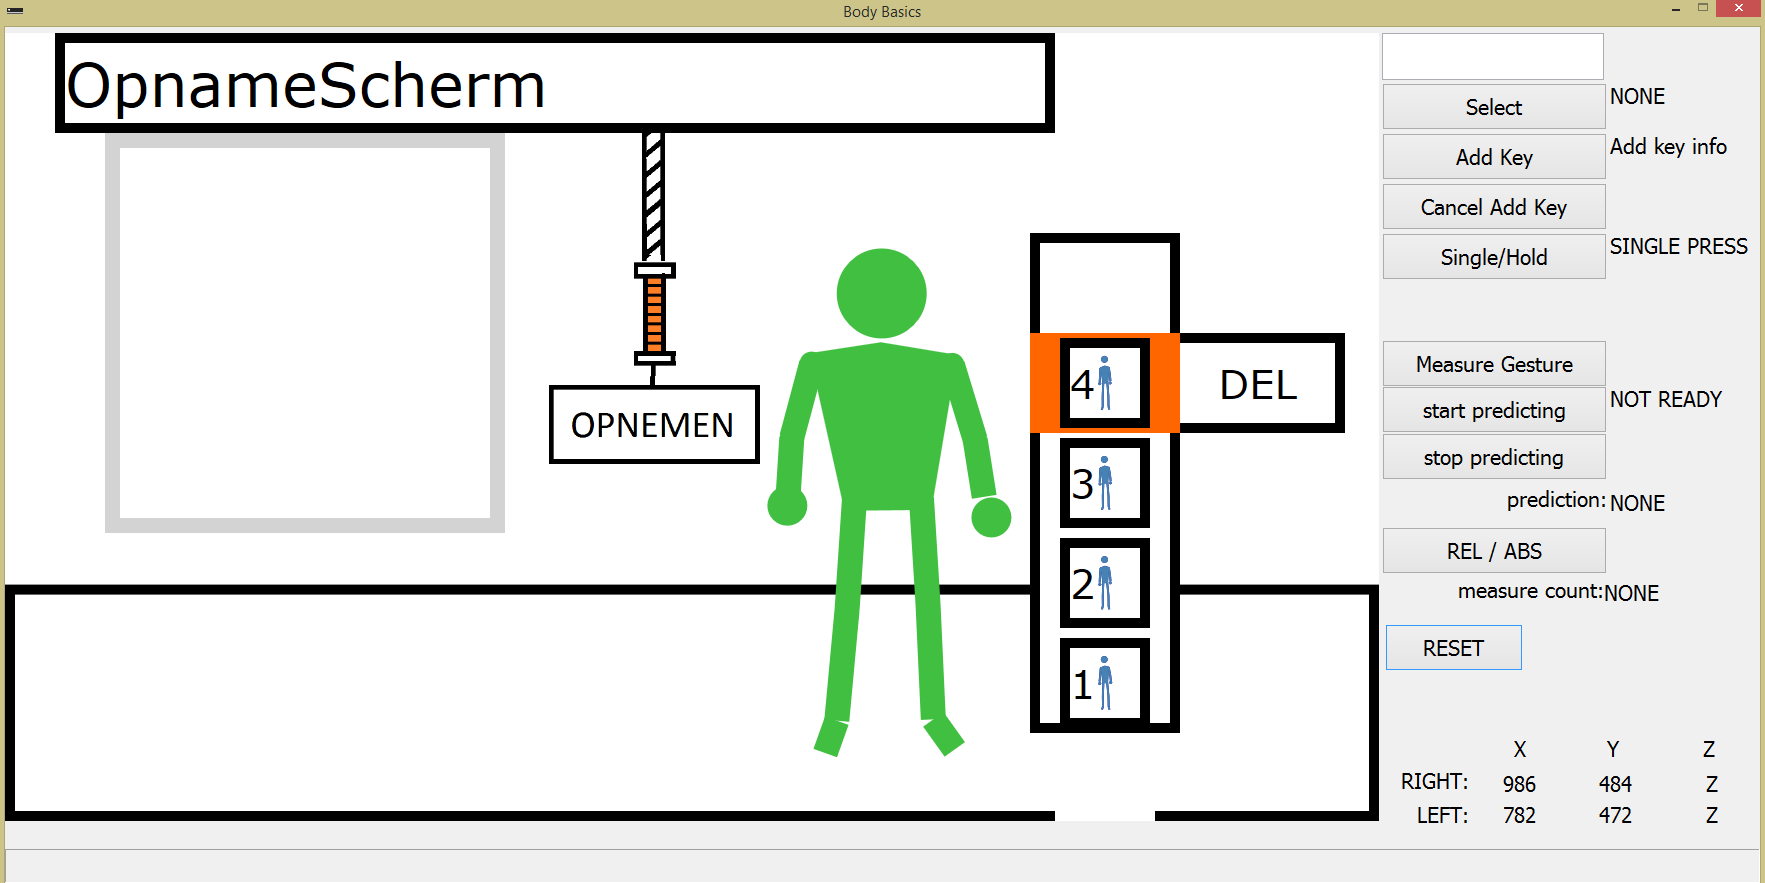
\includegraphics[width=14cm]{figures/1_full_screen_with_user.png}
		\caption{\emph{The full screen of the program}}
		\label{real implementation}
	\end{center}
\end{figure}

\subsection{Class diagram}

The program is build out of an uncopyrighted example by Microsoft called \emph{BodyBasics-D2D} that contained all code to draw 2D skeletons of people seen by the Kinect camera on an empty background. The original program had all of its code centered into one class but has been refactored into a more defined structure as is seen in Figure \ref{fig: gui_classdiagram}. The original code has been spread over the Main, UI, Model and D2D\textunderscore Graphics into a Model-View structure with the Main class initiating the resources for the Kinect, creating the UI and Model class and starting the program loop. The UI received all the elements retaining to the view and controller, while the model received all code retaining to the processing of the Kinect input. The D2D\textunderscore Graphics serves as an interface between the UI classes and the D2Direct canvas.

\begin{figure}[H]
	\begin{center}
		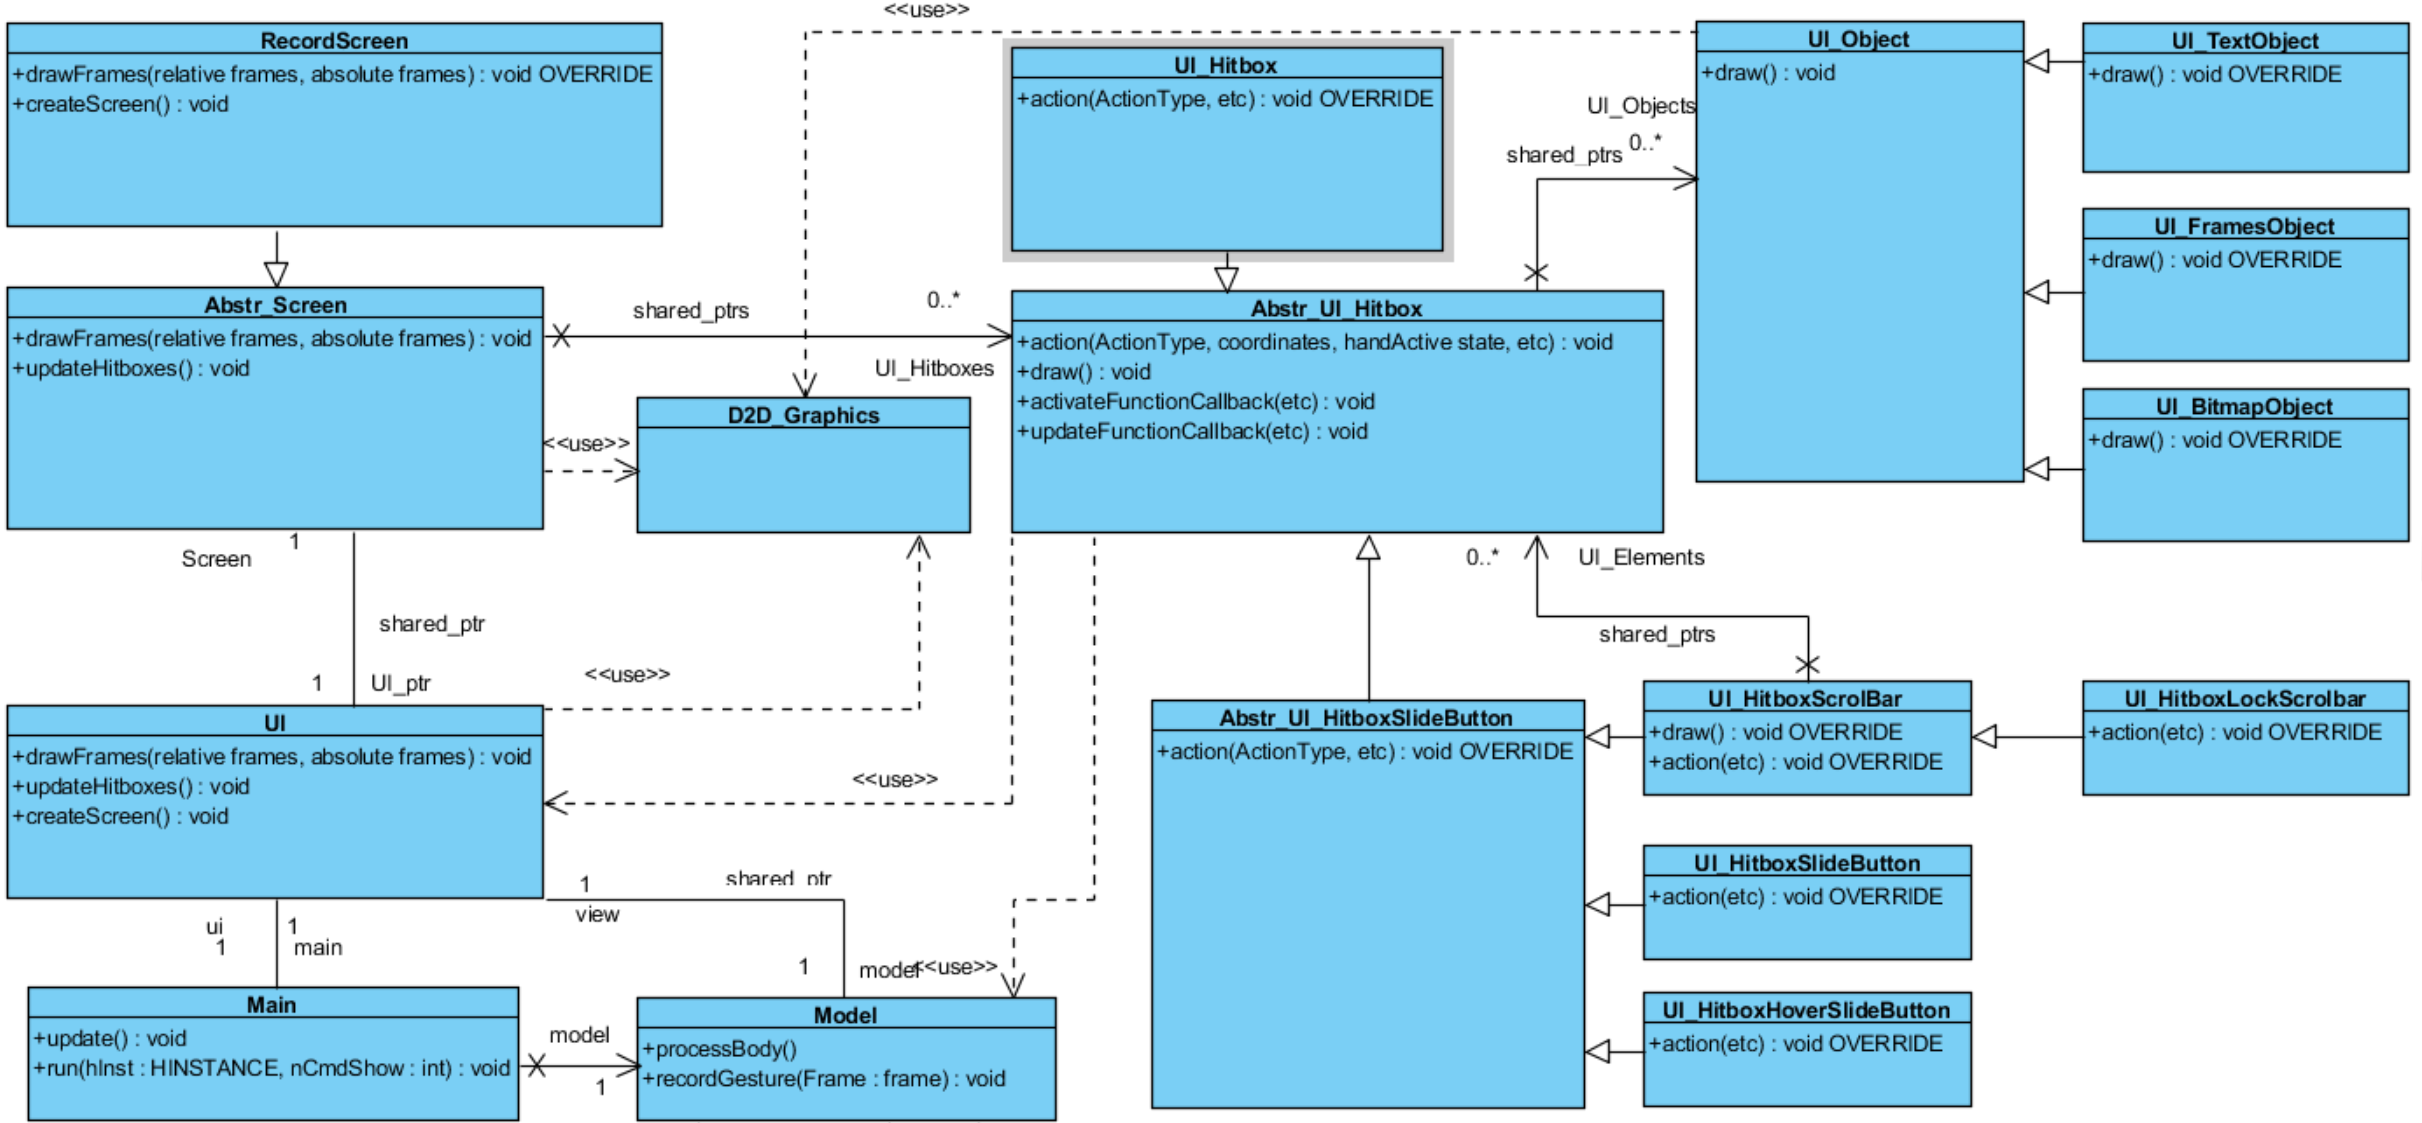
\includegraphics[width=14cm]{figures/UML_UI.png}
		\caption{\emph{The class diagram of the application, focusing on the GUI}}
		\label{fig: gui_classdiagram}
	\end{center}
\end{figure}

The UI class is the main class for the UI part of the program. It serves as the main manager of the view and controller related classes and is the only one through whom the Model class can activate UI elements. It creates the main window in which the application is displayed and handles the input from the WPF UI elements and the keyboard input. At construction a global instance of the D2D\textunderscore Graphics class is created so that all other classes can have direct access to the screen. It also initializes the resources for the D2Direct canvas. It contains a pointer to the current screen that is displayed, every time a new screen is opened the object of the old screen is freed and replaced with a new object of the current screen. This class is responsible for creating the instance whenever a new screen is opened. Though at this point there is only one screen so the pointer is never changed. Three important functions are:  drawFrames(), UpdateHitboxes(), createScreen(). drawFrames() manages the D2Direct resources and starts and ends the drawing on the canvas of D2D\textunderscore Graphics and also passes the draw command to the Abstr\textunderscore Screen class, it is called by the Model class to redraw the screen. UpdateHitboxes() is used by the Model whenever changes in de model data need to be displayed in the UI it is also passed on to the Abstr\textunderscore Screen class. The createScreen() method is called by the Main class when all resources are initialized and the Model is created, the UI class passes it on to the Abstr\textunderscore screen class to instruct it build the elements for the current screen.

The D2D\textunderscore graphics class contains methods from the original example program, methods to initialise the D2DResources, to convert 3D joint coordinates to 2D screen coordinates and to draw the body, though some of these methods were adjusted to our preferences. It also contains new methods to draw Bitmaps, Text or scale 2D skeleton coordinates to different sizes. 

To explain the rest of the structure it is necessary to start with the simplest class and work our way up to the bigger classes.

The UI\textunderscore Object class and its children are an undisputed part of the view organized in a kind of strategy pattern in which each child adds properties and defines the draw() function differently. It contains information about how a rectangle element is drawn using a center, width, height format whilst also containing additional properties such as color, border color and border thickness, etc. The most important function is draw() that uses the D2D\textunderscore Graphics to draw their rectangle. As mention before, each child class overwrites this function to draw their own specific type of image.

The UI\textunderscore TextObject class is a child of the UI\textunderscore Object class that is used to draw text on the D2D\textunderscore graphics. It contains only the necessary properties of the text. The rectangle within which the text is drawn is defined by the parent class.

The UI\textunderscore FrameObject class is also a child of the UI\textunderscore Object class that is used to draw images of puppets other than the one directly controlled by the user.The puppet is scaled to the dimension of the rectangle defined by the parent class.

The UI\textunderscore BitmapObject is the last child of the UI\textunderscore Object class that is used to draw bitmaps scaled to the dimensions of the rectangle defined by the parent class. This is the only object that uses states to decide which image is drawn. Three states are defined : standard, hover and handActive. Standard behavior is to draw the standard image for all states, but each state can be assigned to a different image.

The Abstr\textunderscore UI\textunderscore Hitbox class represents a rectangle that takes on different states dependent the position and state of the hands of the user. The different states that the class can attain are: "hover" when a hand is hovering over the borders of the defined rectangle, "handActive" when the hovering hand is in the activeHand state, such as a closed hand, "activeHandOutside" state when the user's hand moves outside of the rectangle while the hand is in the activeHand state. The states are indicated by flags in the class. The action(etc) function defines behavior for the entering, holding and leaving of a each state using enums. Additional flags allow the usage of special circumstances such as when the hand enters the rectangle while in the activeHand state. This action(etc) function is the main function that is redefined by every child to obtain more complex behavior using these states. This means that every hitbox that has a different effect on the UI most have his own class that is a child of this class. This is the reason why the strategy pattern is used. The class contains a vector of shared pointers to UI\textunderscore Objects upon which the class can act, like move them or change their color and which is used to instruct the UI\textunderscore Objects to draw themselfs when the method draw() is called. Multiple hitboxes can have a pointer to the same UI\textunderscore object so they can all change it. It also contains two callback functions, one is called the activateFunctionCallback which defines the action performed on the Model and UI when the criteria for activation of the hitbox have been reached and one the updateFunctionCallback which defines the behavior when the data in the Model is changed and the UI is updated accordingly.

The UI\textunderscore Hitbox class is a child of Abstr\textunderscore UI\textunderscore Hitbox and as mentioned before it redefines the action method to define a specific behavior when entering,holding and leaving each state. This type of hitbox will change the color of all his UI\textunderscore Objects when the user hover over it and again when the user enters the activehand state while hovering, such as closing his hand. In the former situation the activation callback function is also called. No instance of this object is currently used in the interface.

The Abstr\textunderscore HitboxSlideButton class is a different abstract class that adds behavior to the parent class. Specifically it adds functions to calculate how far the hand that is interacting with the hitbox has moved since the last frame. This information can be used in its children to move hitboxes and UI\textunderscore Objects relative to the hand's movement. Parameters within this class define how far the hand can move from the hitbox's original position and when the activation callback function is called.

The UI\textunderscore HitboxScrolbar class adds a vector of Abstr\textunderscore UI\textunderscore Hitboxes and uses the behavior defined in UI\textunderscore HitboxSlideButton to move them up or down according the movement of interacting hand. \\
{\large COMMENT: redefinition of the draw method} \\

The UI\textunderscore HitboxLockScrolbar class adds the act of locking each Abstr\textunderscore UI\textunderscore Hitboxes derived object in its vector into predefined positions when the user stops scrolling. It also manage the behavior of the orange selection box as discussed in the previous chapter where this class of hitbox is used as the scrollbar in the end design.

The UI\textunderscore HitboxSlideButton defines behavior to slide a button until an activation point is reached. In this specific case the user has to put his hand into the handActive state, before he is able to slide the button. The rope described in the chapter \textbf{Reference!} is an instance of this class.

The UI\textunderscore HitboxHoverSlideButton basically does the same as the UI\textunderscore HitboxSlideButton but doesn't require the user to put his hand into the handActive state. A hand hovering in any state on the right side of the hitbox rectangle will begin sliding it towards the activation point. This class is used in the chapter \textbf{Reference!} as the delete slide button for the recorded elements in the scrollbar.

The Abstr\textunderscore Screen class is an abstract class for the creation of different screens. It holds a vector of shared pointers to all hitboxes on the screen, defines how the puppet of the user is drawn and provides functions to draw background and top UI elements to be defined by his children. For every different screen a new child of this abstract class needs to be added.

The RecordScreen class is a child of Abstr\textunderscore Screen that defines the type and the properties of the hitboxes and UI\textunderscore hitboxes that are used to create the screen as it is described in the previous chapter. The hitboxes are also given their callback functions that are used when the hitbox is activated and when the Model calls for an update of the UI representation.

\subsection{Flow of the program}

The general flow of the program is that at the start of the program, after the creation of the UI and Model objects, the UI class object is instructed to fill his pointer to the Abstr\textunderscore Screen class with an instance the RecordScreen class and then call the function createScreen() on it to create all the hitboxes and UI\textunderscore objects that belong to that particular screen. Then the program loop is started and the processBody() method in the Model class calls the DrawFrames(etc) method in UI which will pass it on to its pointer of Abstr\textunderscore Screen now pointing to a RecordScreen object. This will first call the draw() method on all the hitboxes belonging to the background, which will recursively pass on the draw() function to any Abstr\textunderscore UI\textunderscore Hitbox child or UI\textunderscore Object child it contains. At this stage only the UI\textunderscore Object class and his children will actually call the D2D\textunderscore Graphics object to draw something on the Direct2D canvas. Then drawFrames (etc) function continues by calling the D2D\textunderscore Graphics object to draw the puppet representing the user and on top of that the hitboxes of the top UI are drawn in the same manner as the background. Last the coordinates and states of the hands of the user are given to every hitbox in the screen, these will use this information to determine and execute any changes in their state or their UI\textunderscore objects based on their criteria. If a hitbox determines that his activation criteria have been met he calls his activateFunctionCallback(etc) that will make calls directly to the Model. This happens every cycle when the processBody() function in the Model class is called, which is usually 30 times per second.

Whenever something changes in the Model structure that affects the representation in the UI, a flag is set and during proccesBody() the updateHitboxes() function is called on the UI object before the UI is drawn. The UI passes this on the Abstr\textunderscore Screen child who calls an update() function on all the hitboxes it contains. Each hitbox will call their own updateFunctionCallback(etc) to retrieve all information related to them from the Model and process it. Hitboxes that contain other hitboxes will call the update() function recursively.

%TODO klassendiagramma van de GUI + eventuele snippets uit de code (+ uitleg)



\section{Back-end software}

\subsection{Class diagram}

The focus of the application is reflected by the structure of the code. The class diagram shows a model-view pattern to make a distinction between the graphical interface of the application and the back-end (see figure \ref{fig: backend_classdiagram}).\\

\begin{figure}[H]
\begin{center}
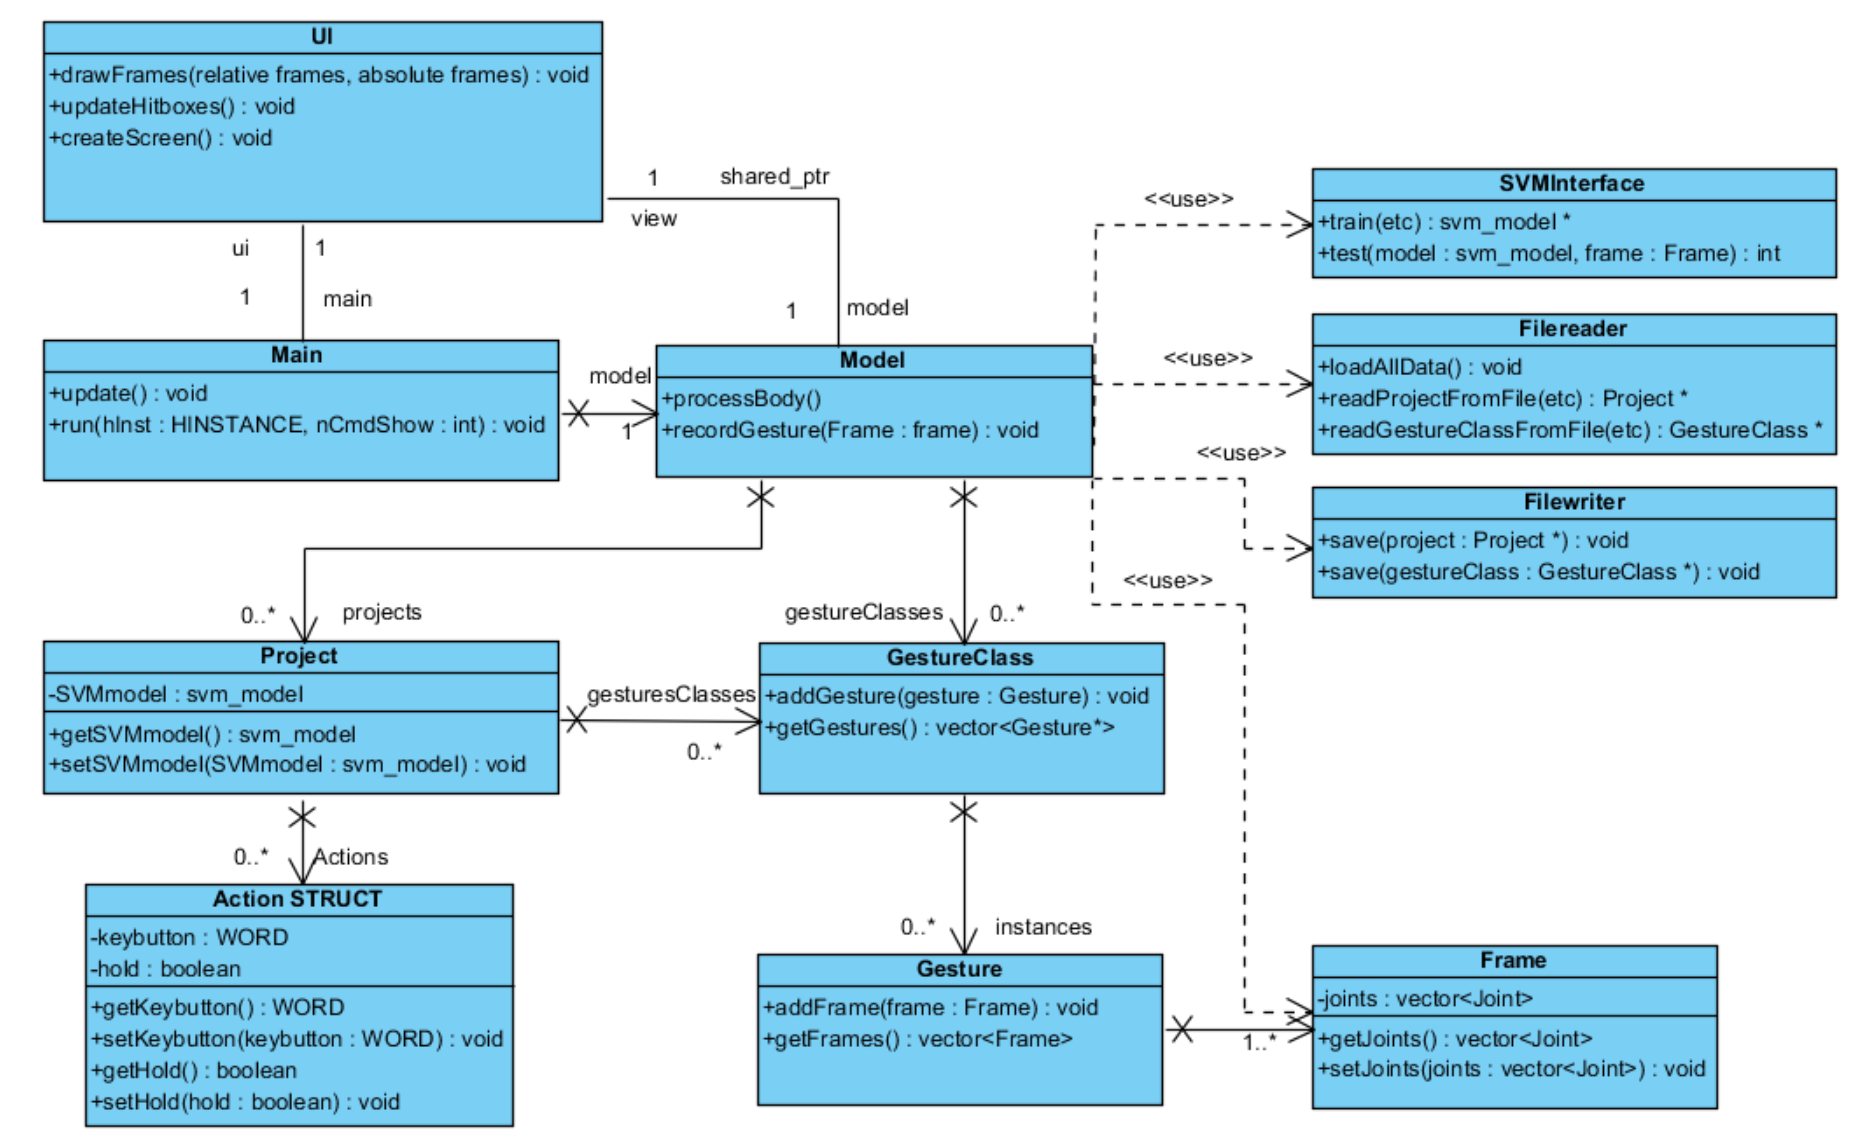
\includegraphics[width=14cm]{ClassDiagramBackEnd.png}
\caption{\emph{The class diagram of the application, focusing on the back-end}}
\label{fig: backend_classdiagram}
\end{center}
\end{figure}

The Kinect camera has the ability to identify and measure the position relative to the camera of 25 points of a person, for instance: left elbow, right elbow, head, center of the spine, left wrist,\ldots All of these points are referred to as \classname{Joint}s and can be accessed using the libraries that come as part of the Kinect SDK installation. Each \classname{Joint} has an $x$, $y$ and $z$ coordinate, so it is unambiguously defined in space.\\

When the Kinect measures all of the \classname{Joint}s at one specific point in time, these 25 \classname{Joint}s together form one frame. This can be seen as a single picture of a person taken by the camera. Analogous to a movie, which is nothing more than a quick succession of pictures, an instance of \classname{Gesture} collects all \classname{Frame}s, which all together, contain information about how the person moved over a period of time.\\

In order to improve the application's ability to recognize an exercise, each of the exercises must be trained more than once by the physical therapist. For each exercise that is trained, an instance of \classname{Gesture} is created. The \classname{Gesture}s that contain data about different executions of the same exercise are grouped into a \classname{GestureClass}. In other words, one \classname{GestureClass} object contains all trainings of the same exercise.\\

After setting up a \classname{Project} object, it contains all data that is needed for playing a game using the application. It has a \classname{map} that maps a label for each exercise to a \classname{GestureClass} and the actions linked to that \classname{GestureClass}. An \classname{Action} contains information about the keyboard key that needs to be pressed and if that key should be held down or be quickly pressed and released. The \classname{Model} class forms the core of the application. It controls the flow of the program and contains all important objects, such as the \classname{Project} and the \classname{GestureClass}es. By storing the \classname{GestureClass} objects in \classname{Model} rather than \classname{Project}, it is possible to reuse the same \classname{GestureClass}es in multiple \classname{Project}s.\\

\classname{SVMInterface} takes all gesture data and converts it to a format that is accepted by the LibSVM library \cite{LibSVM}. This is an existing library that provides a C$++$ support vector machine implementation and is used in this application for gesture recognition.\\

To prevent having to train all exercises again each time the application is started, all necessary data is saved into files in the data folder using the \classname{Filewriter} implementation. This includes the data of the \classname{Gesture}s, \classname{GestureClass}es, \classname{Project} and the computed SVM model. The \classname{Filereader} is responsible for reading data from the saved data files when the application is started.\\


\subsection{Flow of the program}

After initialization of variables like the instances responsible for the user interface and the communication with the Kinect camera, the program locks into an infinite loop while the application is running. This main loop consists of three processes: fetching new data from the Kinect camera, analyzing this data in order to use it for recording or predicting gestures and updating the GUI with relevant changes.\\

It is important that none of these three processes block the continuous flow of the main loop. The update rate of the interface is only as fast as the rate with which the main loop is executed. If it is slowed down with a blocking or long-running loop, the GUI appears to stutter or freeze and no new data is collected from the Kinect camera.\\

The Kinect can only provide new data as fast as 30 times per second. If no new data is available at the moment the main loop requests the data, for instance when the main loop is executed faster than 30 times per second, the program skips this process and continues with the other two processes.\\

To control the flow of the program without reverting to blocking loops, software flags are used. These flags keep track of the current state of the program. By evaluating the state of the flags, it is possible to indicate if the program is predicting a gesture, recording a gesture or animating specific graphical elements of the GUI.


\section{Gesture recognition}

It is possible to split up the implementation of gesture recognition into two parts: the recording of a gesture by the physical therapist and the prediction of a gesture executed by a patient.


\subsection{Recording a gesture}

Code snippet \ref{code_record_gesture} shows the code for recording a gesture. When the recording of a gesture is initialized, the first frame is stored for reference. Actual recording starts when the users starts moving. This means that the first frame is different from the current frame. Two frames are considered equal when all of the joints of both frames in all three dimensions have a difference of less than 12 centimeters. In other words, if the person moved more than that, the frames are not equal. The threshold of 12 centimeters is chosen due limitations of the Kinect camera, where small variations in measurements are possible. Additionally, it is hard for a person to stay perfectly still, so the choice of the threshold can eliminate recognizing small tremblings as the user having moved.\\

When actual recording is initialized, the frames are stored in a buffer. Together, the frames of this buffer form an entire gesture. If the buffer is filled up without the user moving, this means that the user is recording a posture rather than a gesture. However, when the user moves, recording can be ended by standing still in an ending position of choice for approximately 1 second.\\

\begin{lstlisting}[caption=method to record a gesture, label=code_record_gesture]
void Model::recordGesture(Frame & frame) {
	if (!initialized) {
		//Set the first frame on the first call
		firstFrame.setFrame(frame);
		initialized = true;
	}

	if (!startedMoving) {
		if (! frame.equals(firstFrame)) {
		
			startedMoving = true;
			framesBuffer.clear();
		}
		else if (framesBuffer.size() > NOT_MOVING_FRAME_DELAY) {
			addRecordedGesture();
		}
		else {
			return;
		}
	}
	
	//Add the frame to the buffer
	framesBuffer.push_back(frame);

	if (framesBuffer.size() > NOT_MOVING_FRAME_DELAY &&	framesBuffer.back().equals(framesBuffer.at(framesBuffer.size() - NOT_MOVING_FRAME_DELAY))) {
		addRecordedGesture();
	}
}
\end{lstlisting}


\subsection{Predicting a gesture}

Code snippet \ref{code_gesture_executed} shows a method for predicting a gesture. This method is called recursively. Gestures are split up into a number of smaller parts, referred to in the code as \classname{NB\textunderscore OF\textunderscore LABEL\textunderscore DIVISIONS}. If this constant equals four, it means that a gesture is split up into four parts. For instance, if the base label of a gesture equals one, predictions for labels one, two, three and four all relate to one of the parts of the gesture.\\

Continuing with this example, if during prediction a part of a gesture with label four is found, the recursive method \classname{isGestureExecuted} is called. It checks if shortly before label four is found, label three is predicted as well. If label three is predicted, the method is called recursively to check for label two. This goes on until the base label is reached. At this point, the recursion is ended and the gesture is recognized as being successfully executed. All parts of the gesture must be executed in the right order and fast enough. If the gesture is executed too slow, the buffer with predicted labels is cleared.\\

The method allows that one label is not predicted correctly. There are many reasons this can happen, such as noisy measurements, the user moving differently or not having trained the gesture sufficiently. In the case of the considered example, if labels one, three and four are predicted, and label two is missing, the gesture is still considered to be executed successfully. This can improve user experience while playing a game, as a gesture has less of a chance of being not recognized wrongfully.\\

\begin{lstlisting}[caption=method to verify if a gesture with given label is executed, label=code_gesture_executed]
bool Model::isGestureExecuted(int checkLabel, int posInBuffer, int recursiveCounter, int badCounter) {
	//The label exists and is linked to a posture.
	if (activeProject->containsLabel(checkLabel) && activeProject->getGestureClass(checkLabel)->getGestures().front()->isPosture())
		return true;

	//Done enough recursive checks to confirm the gesture has been executed.
	if (recursiveCounter >= NB_OF_LABEL_DIVISIONS)
		return true;

	int nextLabelToCheck = checkLabel - 1;
	for (int i = posInBuffer; i >= 0; i--) {
		if (labelsBuffer.at(i) == nextLabelToCheck)
			return isGestureExecuted(nextLabelToCheck, i, recursiveCounter++, badCounter);
	}

	//If this point is reached, a label that is one less than the given
	//	label cannot be found in the buffer.
	//The gesture may still have been executed, so keep checking for the
	//	next one if the badCounter is not too high.
	if (badCounter > 0)
		return false;
		
	return isGestureExecuted(nextLabelToCheck, posInBuffer, recursiveCounter++, badCounter++);
}
\end{lstlisting}